\section{Additional Experiments}
\label{sec:addexp}

\paragraph{CREMI A/B/C.} As part of the MICCAI 2016 challenge on circuit reconstruction from electron microscopy images (CREMI), six ssTEM datasets were made publicly available\footnote{\scriptsize{\url{http://www.cremi.org}}},  each $1250\times1250\times125$ voxels. Since only three datasets include manually-labeled `ground truth', we use these three volumes for our experiments. The volumes are part of an adult fruit fly (Drosophila melanogaster) brain. The resolution of all three datasets is $4\times4\times40~\text{nm}^3\text{/voxel}$. We evaluate error detection and correction on subvolumes of CREMI A/B/C with the dimensions $1250\times1250\times5$ voxels. The subvolumes were cut from the last 25 sections of each of the three datasets and unseen during training. We compare focused proofreading and guided proofreading with automatic selection ($p_t=0.95$) and selection oracle.

\paragraph{Retraining.} Since the CREMI data is a different species, we simply retrain our split error classifier as well as focused proofreading by Plaza~\cite{focused_proofreading}. For this, we use the first 100 sections of each of the three CREMI datasets combined as training data. All parameters are unchanged and left as reported in the paper. 

\begin{figure}[t]
\centering
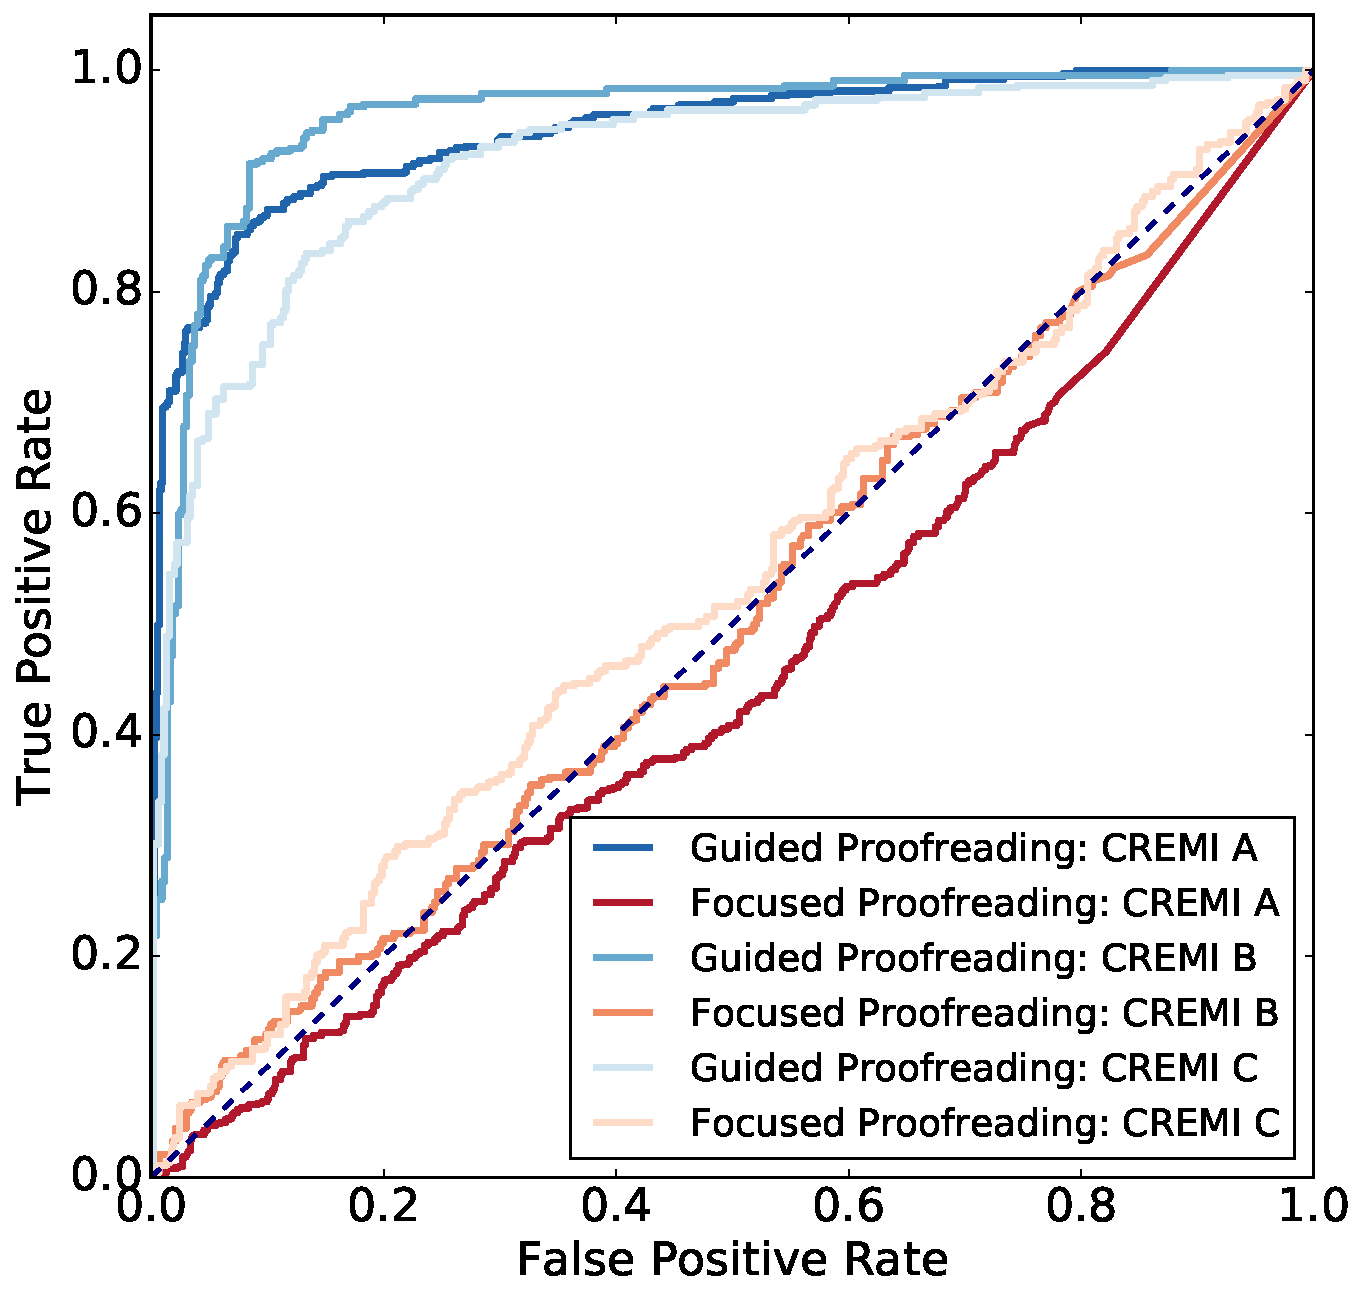
\includegraphics[width=\linewidth]{gfx/cremi_roc_separate_small.pdf}
\caption{Receiver Operating Characteristic curves comparing focused proofreading and guided proofreading automatic correction on the CREMI A/B/C fruit fly subvolumes. Guided proofreading performs better on all three datasets.}
\label{fig:cremi_performance}
\end{figure}

\paragraph{Classification Performance.} Figure~\ref{fig:cremi_performance} compares the  focused proofreading and guided proofreading classifiers on the CREMI A/B/C datasets. Our method exhibits higher sensitivity and lower fall-out.

%\paragraph{Error correction.} In all three datasets merge error detection found over 300 merge errors. Unfortunately, merge error correction crashed because of a software error on our part. Therefore, we only evaluate split error detection and correction on subvolumes of CREMI A/B/C with the dimensions $1250\times1250\times5$ voxels. The subvolumes were cut from the last 25 sections of each of the three datasets and unseen during training. We compare focused proofreading and guided proofreading with automatic selection ($p_t=0.95$) and selection oracle.

\subsection{CREMI A}

\begin{figure}[t]
\centering
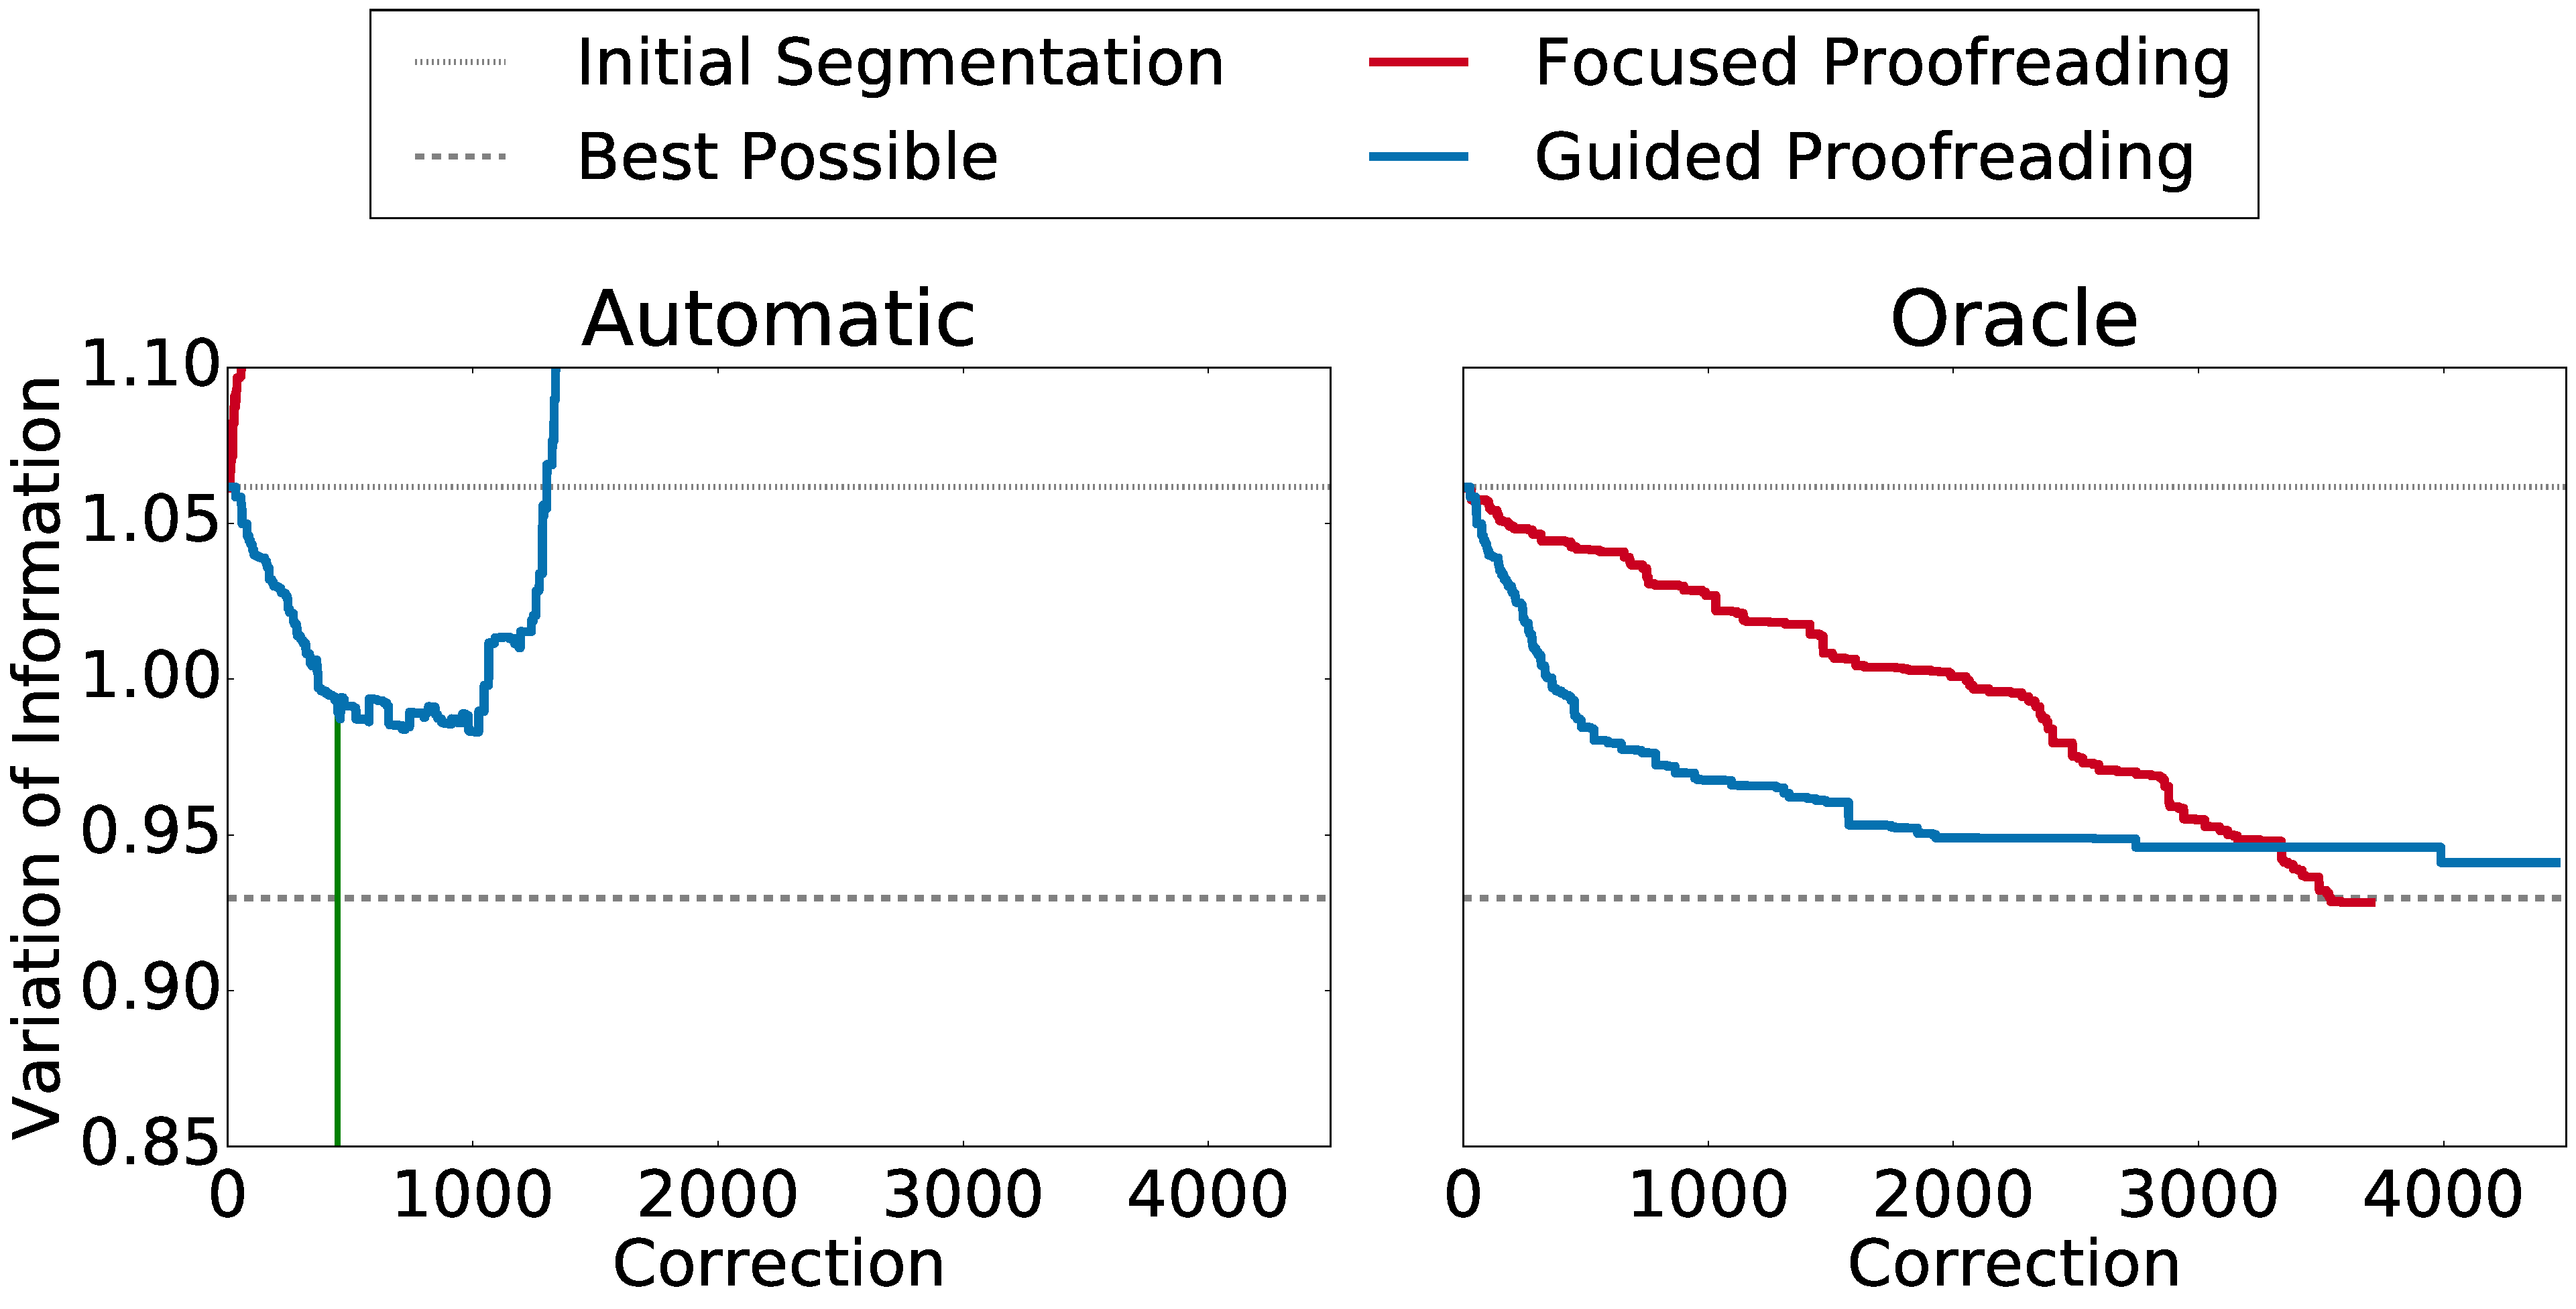
\includegraphics[width=\linewidth]{gfx/cremiA_trails.pdf}
\caption{Performance comparison of Plaza's focused proofreading and our guided proofreading on 5 sections of the CREMI A dataset. All measurements are reported as median VI, the lower the better. The threshold for automatic selection is $p_t=0.95$ (green line). The slope of the selection oracle shows that guided proofreading reduces VI faster.}
\label{fig:cremiAtrails}
\end{figure}

\begin{figure}[t]
\centering
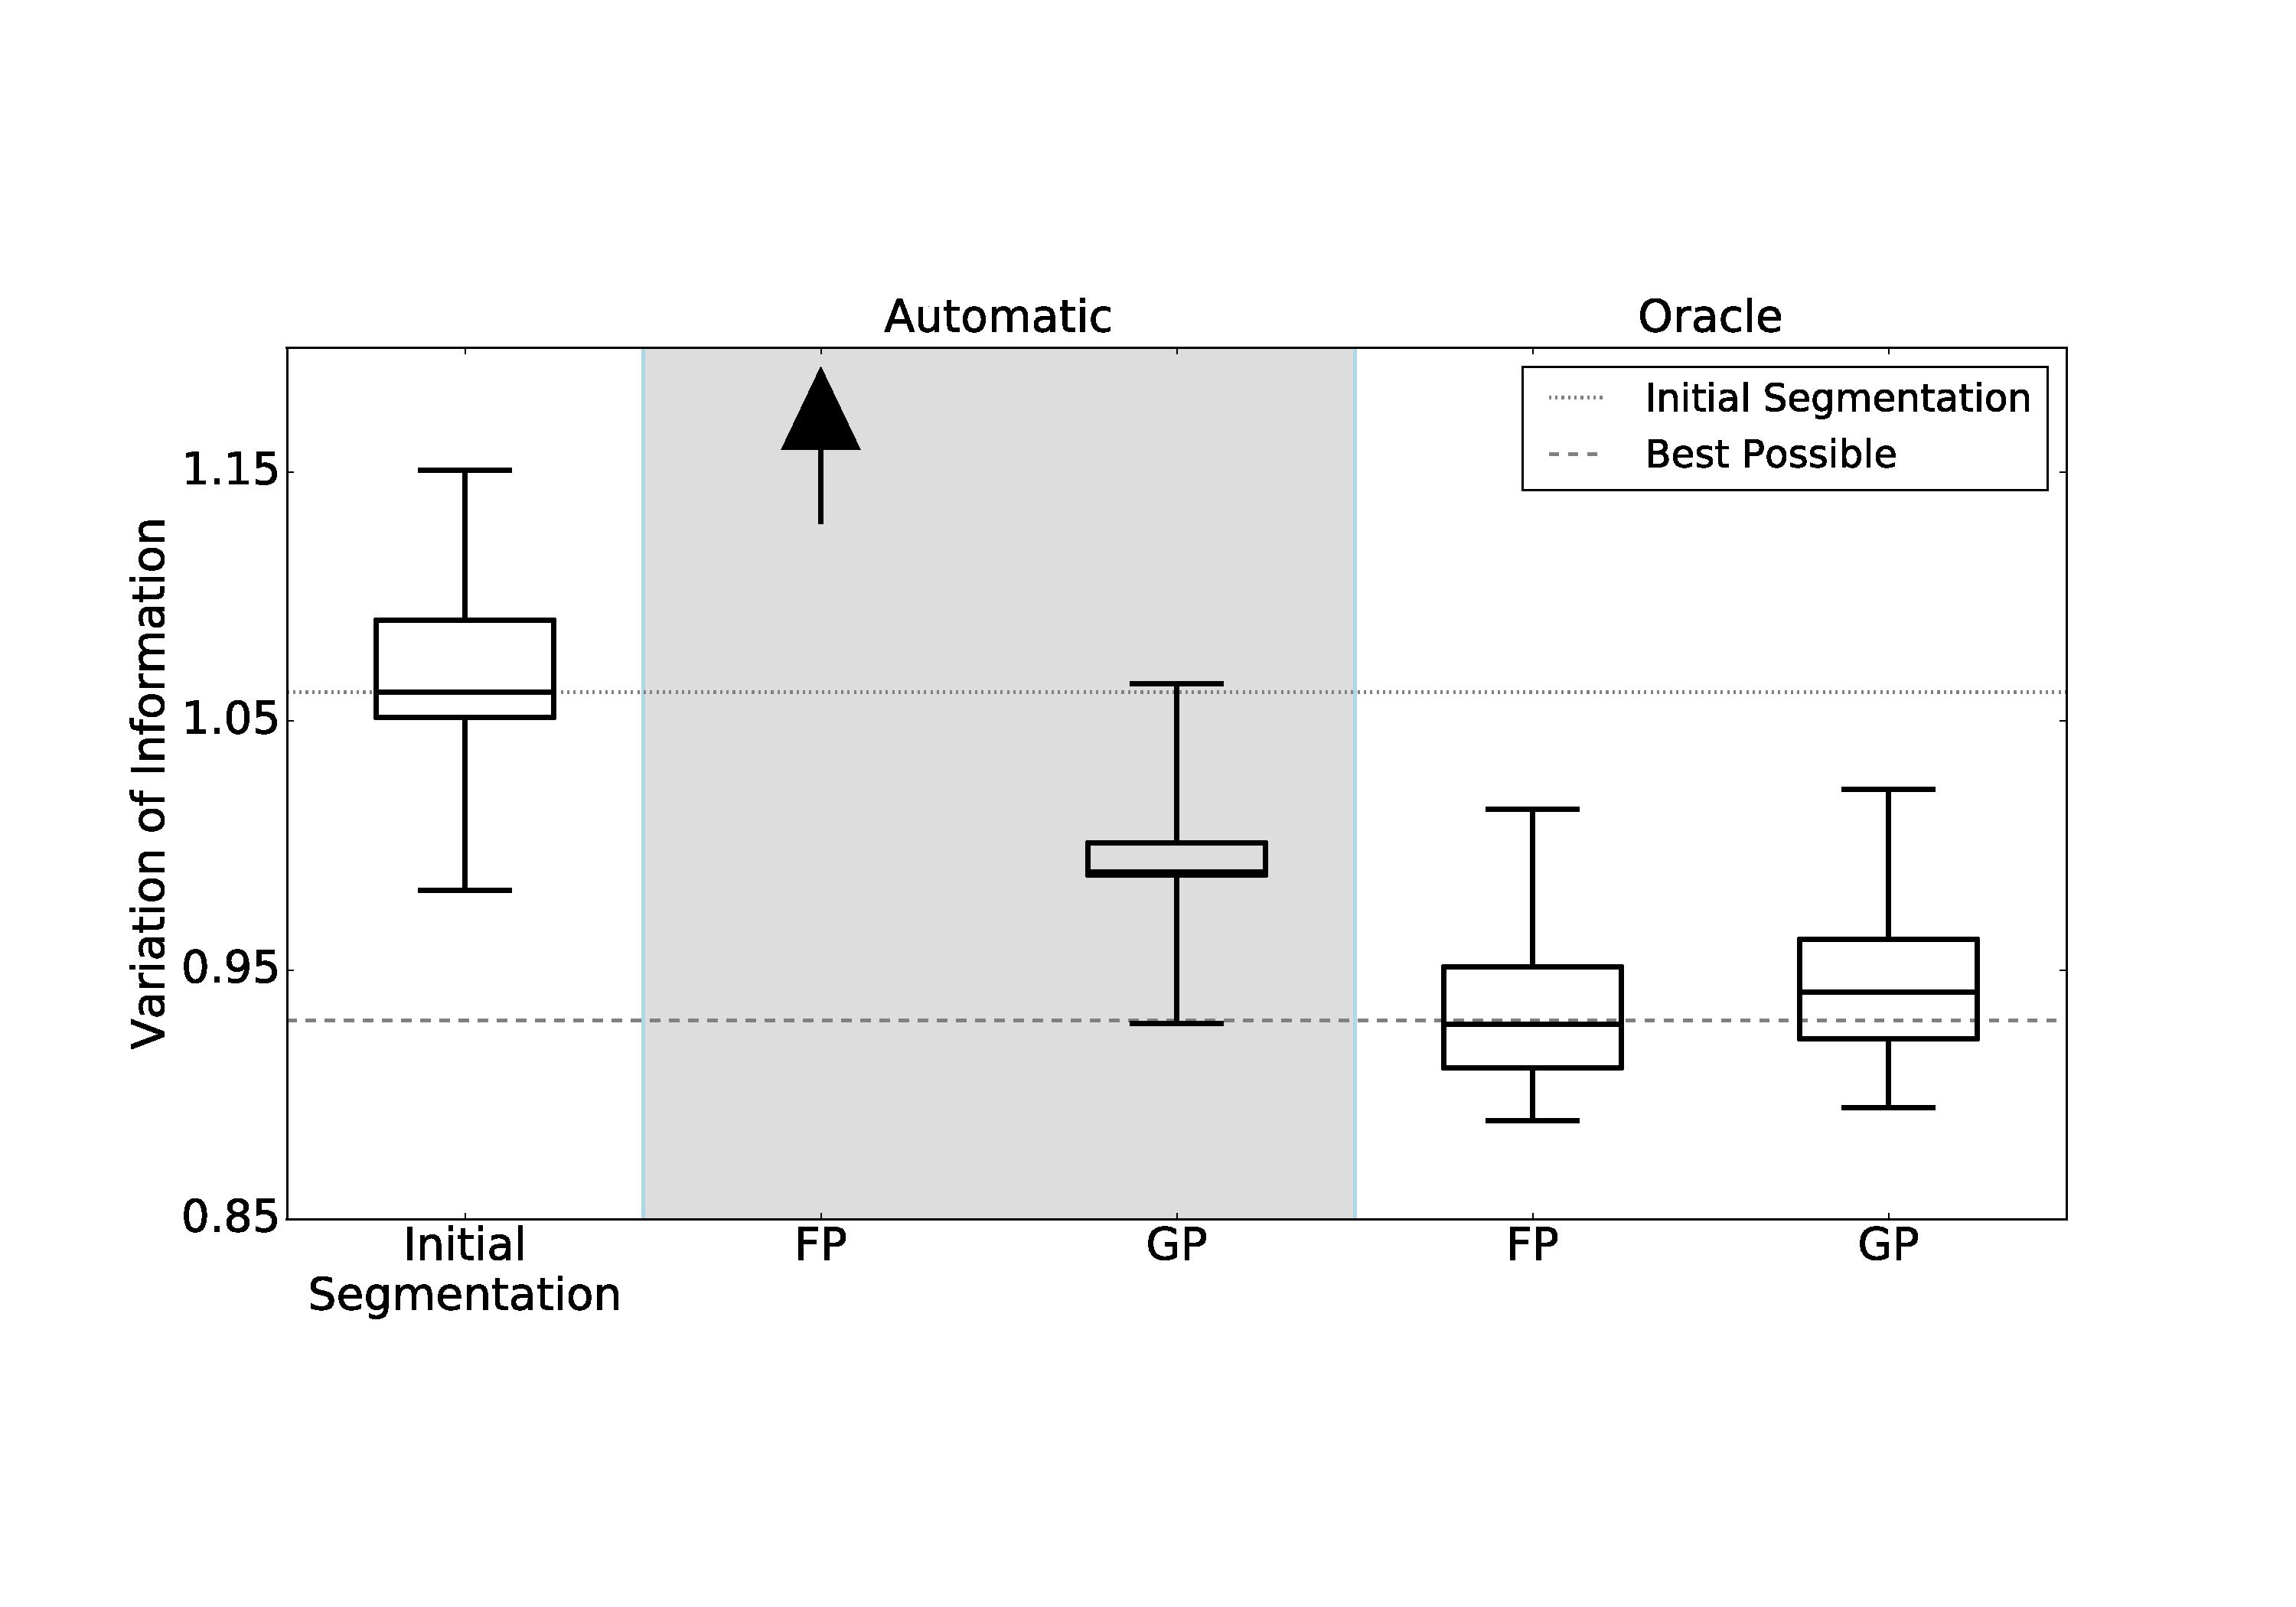
\includegraphics[width=\linewidth]{gfx/cremiAboxplot.pdf}
\caption{VI distributions of guided proofreading (GP) and focused proofreading (FP) output across slices of the CREMI A dataset, with different error correction approaches. The variation resulting from performance of FP with automatic selection is $5.4\times$ higher than GP (\protect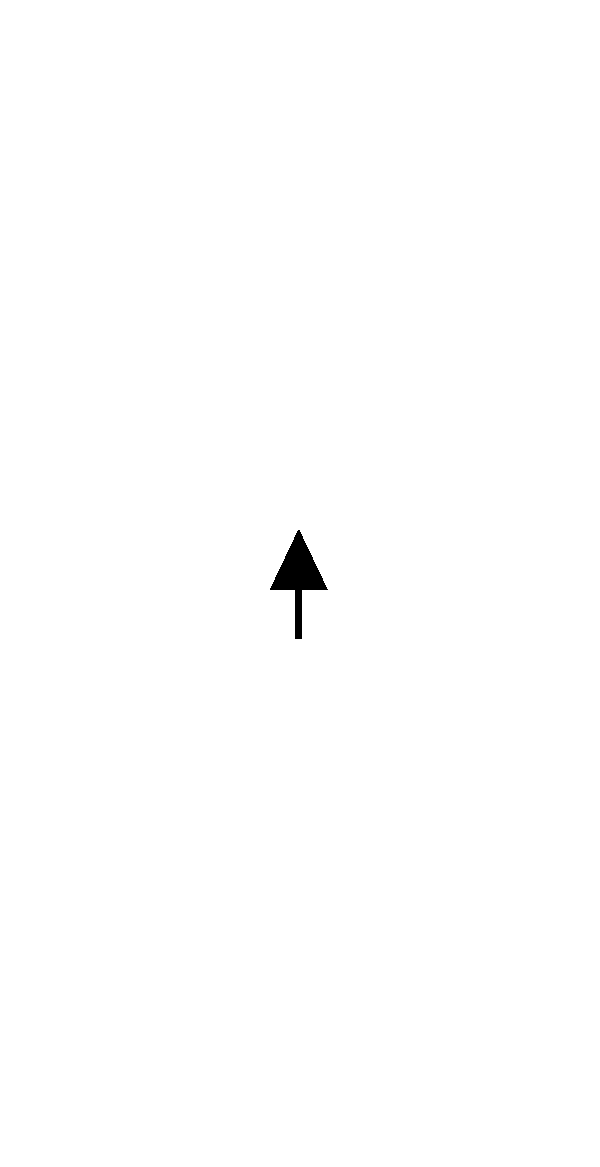
\includegraphics[width=0.2cm]{gfx/arrow.pdf}), with median VI of $5.32$ and $SD=0.009$. GP does not reach the best possible VI as discussed in the text.}
\label{fig:cremiAboxplot}
\end{figure}

Figure~\ref{fig:cremiAtrails} and~\ref{fig:cremiAboxplot} compare Plaza's focused proofreading and guided proofreading on the five sections of CREMI A.

\vspace{-4mm}

\paragraph{Selection oracle.} With focused proofreading, the selection oracle reduces median VI to 0.928, $SD=0.043$ from an initial median VI of 1.06 ($SD=0.055$). 532 corrections out of 3707 were accepted. Guided proofreading does not reach the best possible VI, however, reduces VI faster with less corrections to 0.941 ($SD=0.04$). Out of 4463 corrections, 1275 were accepted.

\paragraph{Automatic selection with threshold.} Not surprisingly, focused proofreading performs poorly when ran automatically (VI of 5.32, $SD=0.009$). Guided proofreading is able to reduce VI to 0.989 ($SD=0.043$) with $p_t=0.95$.

\subsection{CREMI B}

Figure~\ref{fig:cremiBtrails} and~\ref{fig:cremiBboxplot} show the results on the CREMI B dataset.

\paragraph{Selection oracle.} Focused proofreading is able to reduce median VI to 1.29, $SD=0.031$ from an initial median VI of 1.63 ($SD=0.025$). Out of 1959 corrections, the selection oracle accepted 517. With guided proofreading, the median VI is reduced to 1.30, $SD=0.03$ while accepting 1111 corrections out of 3073.

\paragraph{Automatic selection with threshold.} Focused proofreading results in a VI of 4.25 ($SD=0.07$). Guided proofreading reduces median VI to 1.43 ($SD=0.038$).

\begin{figure}[t]
\centering
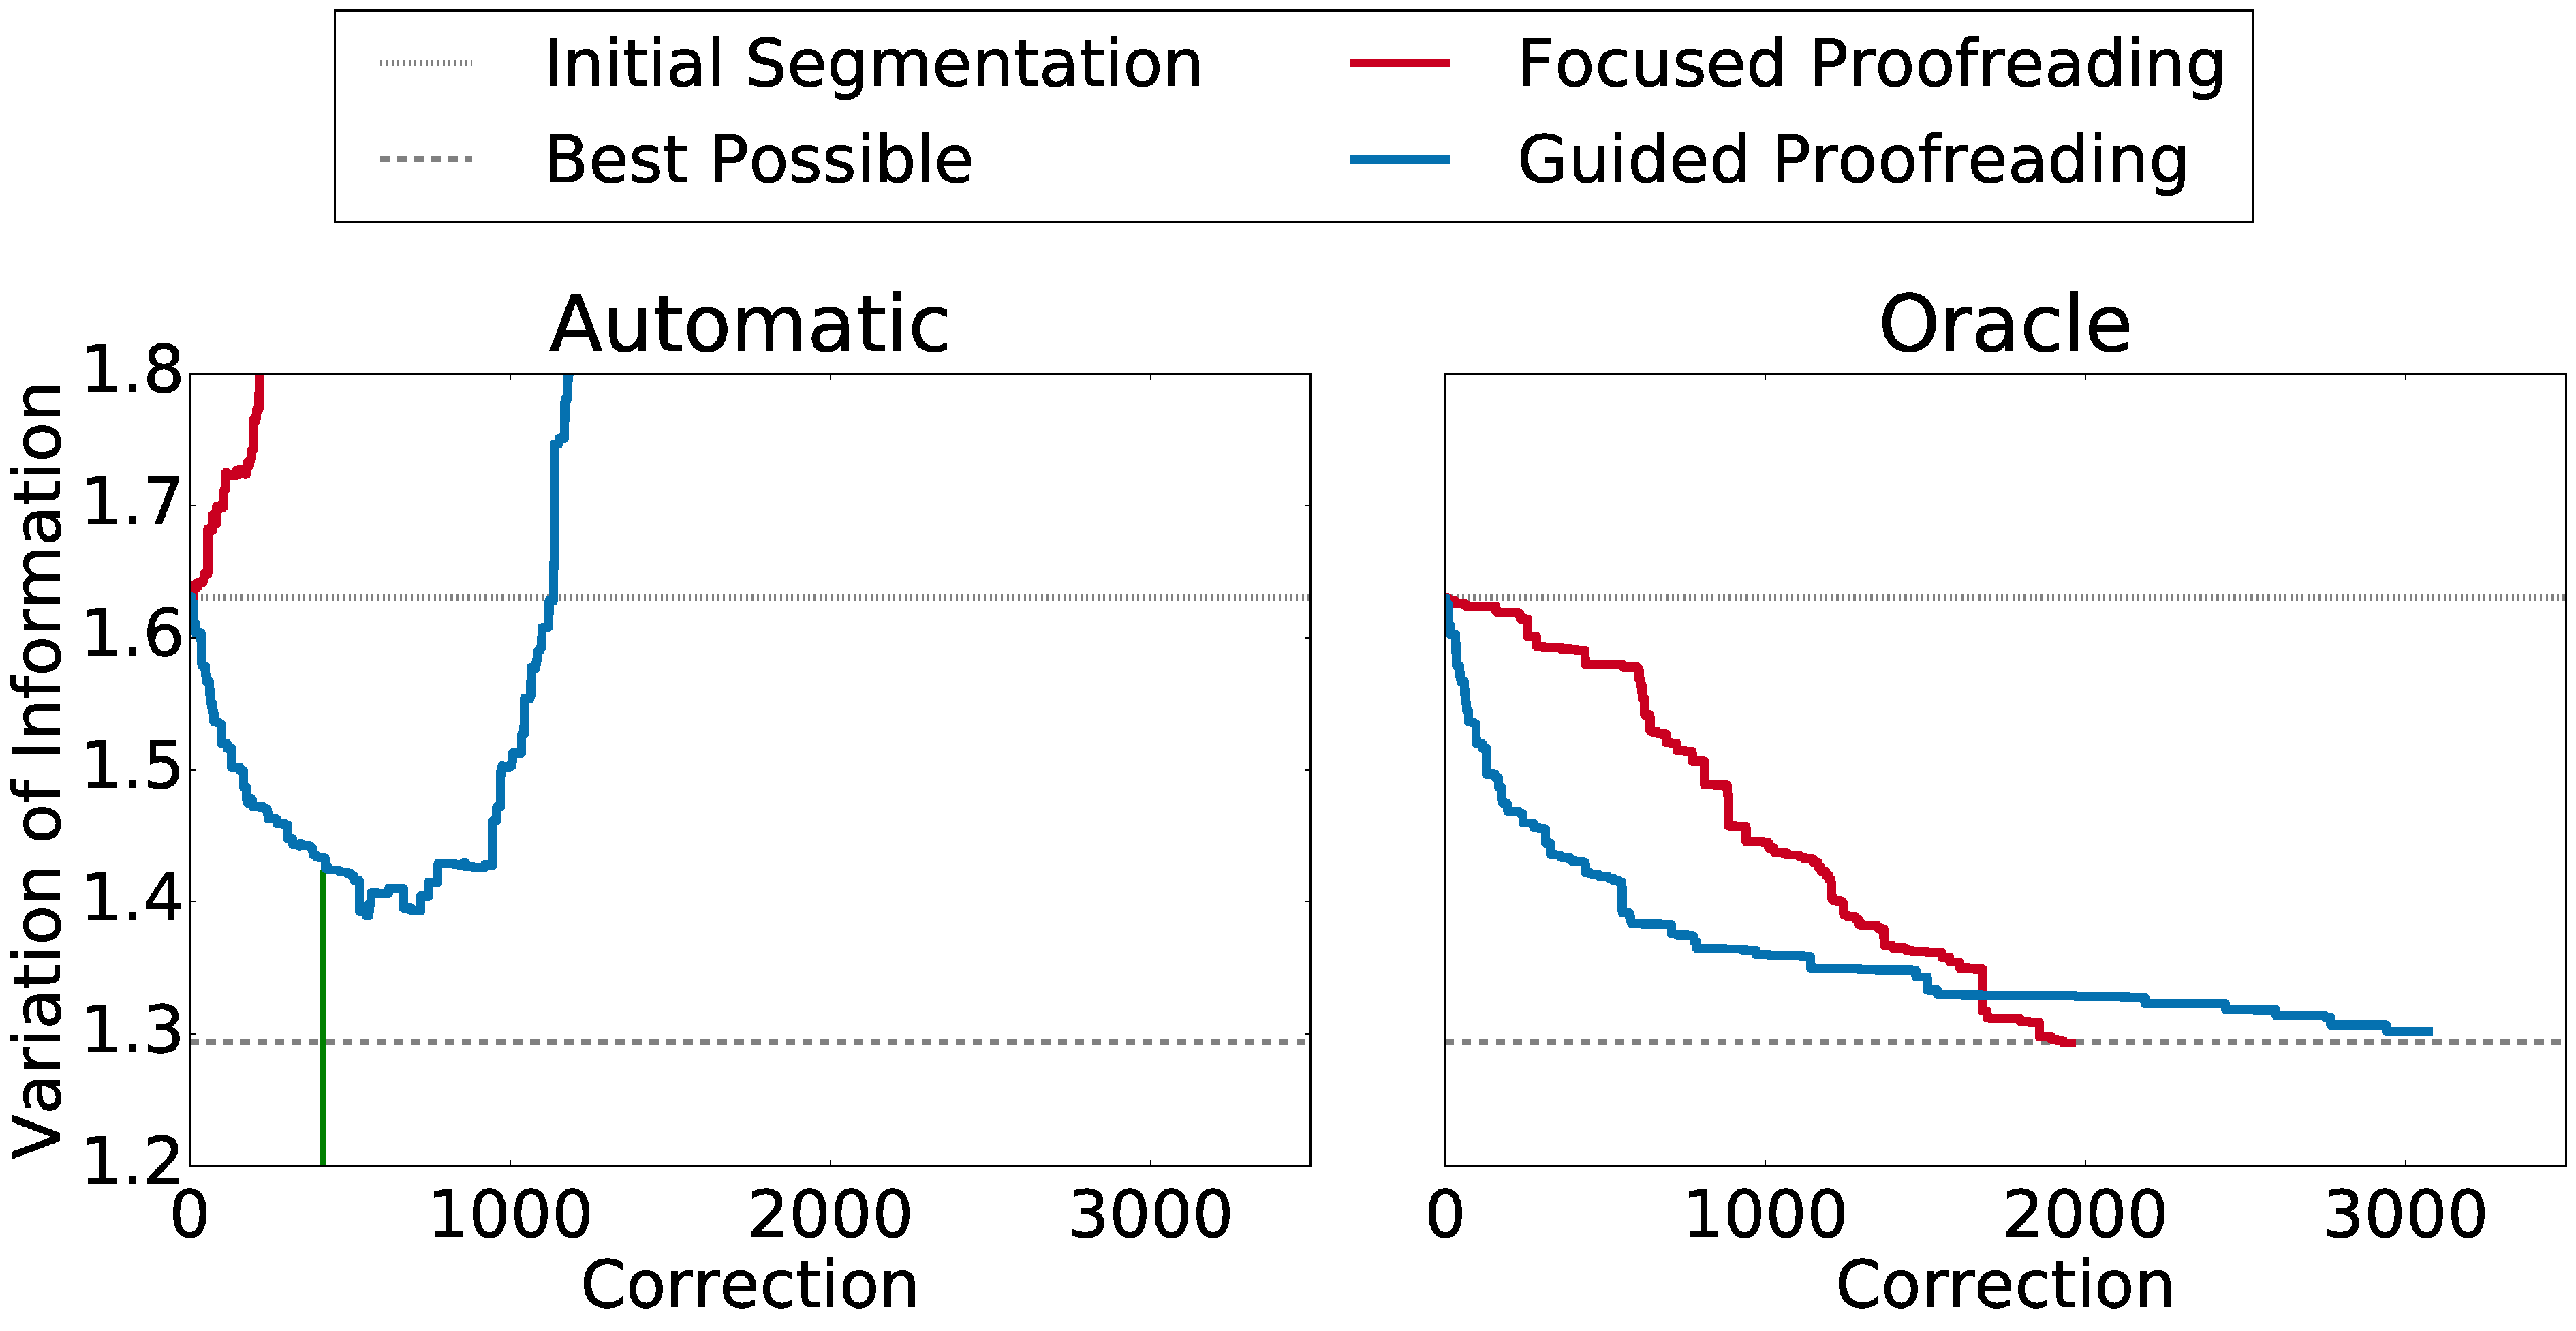
\includegraphics[width=\linewidth]{gfx/cremiB_trails.pdf}
\caption{Split error correction by Plaza's focused proofreading and our guided proofreading compared on the CREMI B dataset. All measurements are reported as median VI, the lower the better. Automatic selection with threshold (green line) yields reasonable performance using guided proofreading.}
\label{fig:cremiBtrails}
\end{figure}

\begin{figure}[t]
\centering
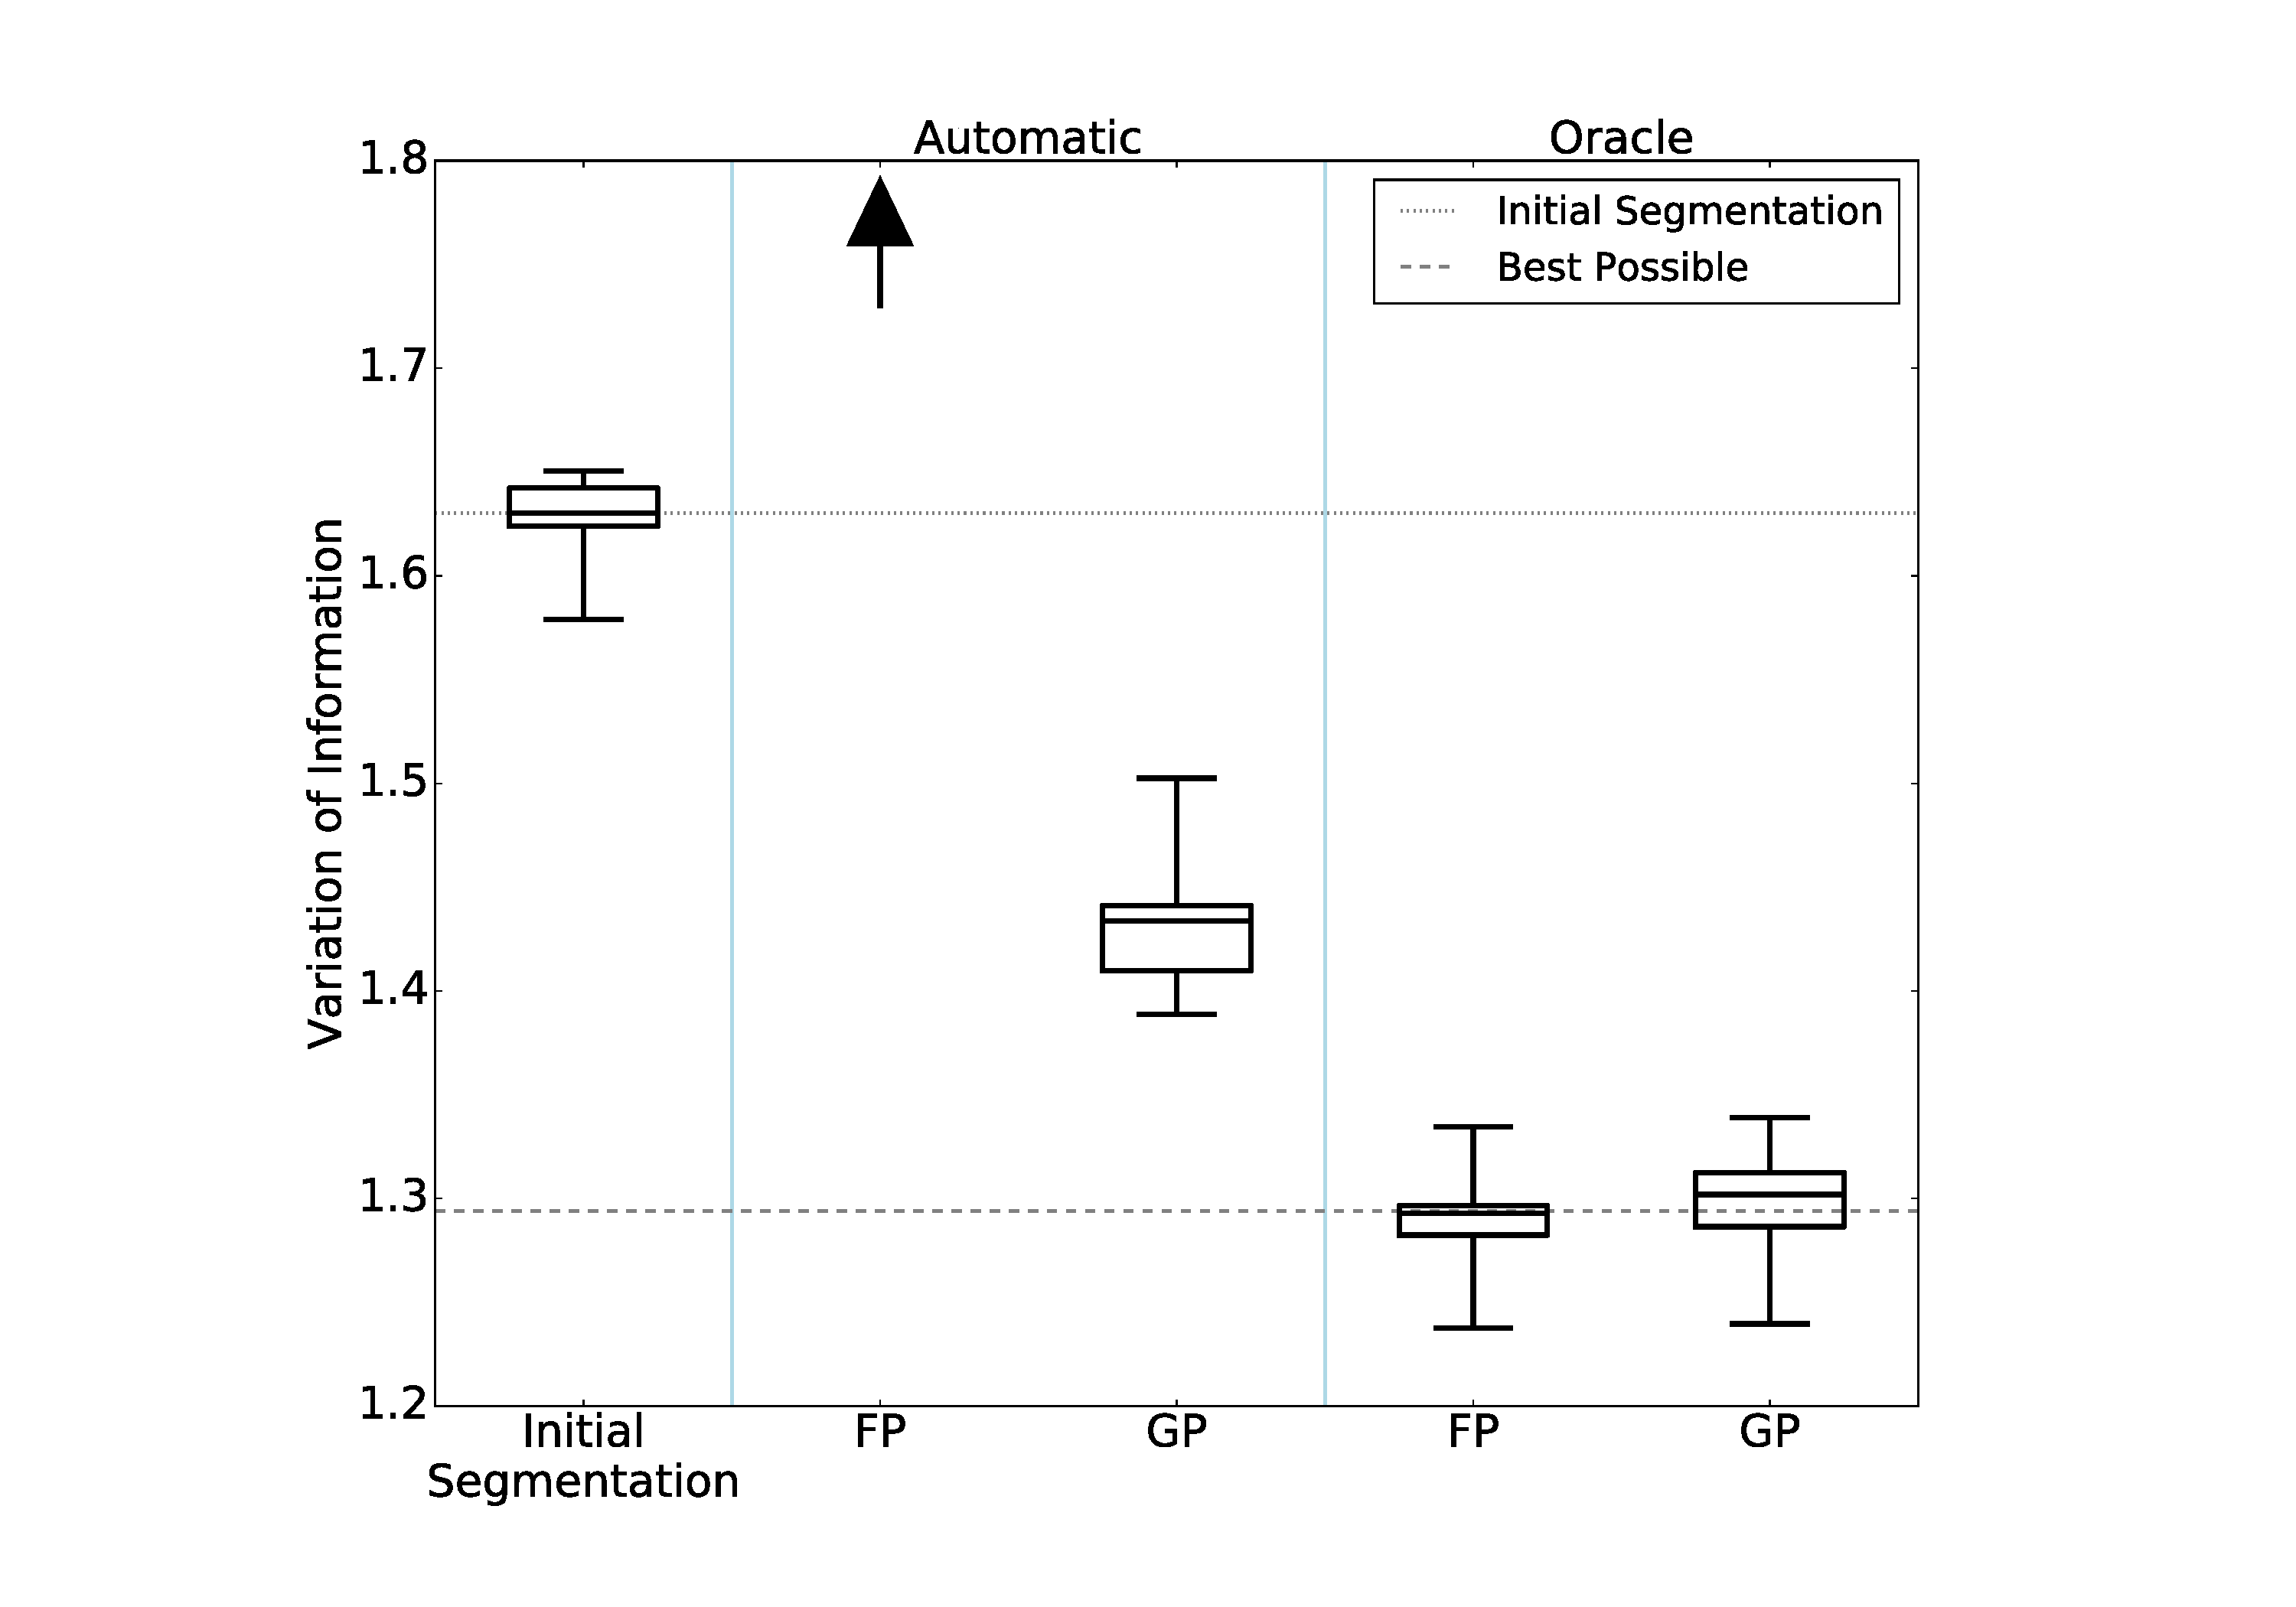
\includegraphics[width=.9\linewidth]{gfx/cremiBboxplot.pdf}
\caption{VI distributions of guided proofreading (GP) and focused proofreading (FP) output across 5 sections of the CREMI B dataset. We compare automatic selection and oracle selection. The variation resulting from performance of FP with automatic selection is $3\times$ higher than GP (\protect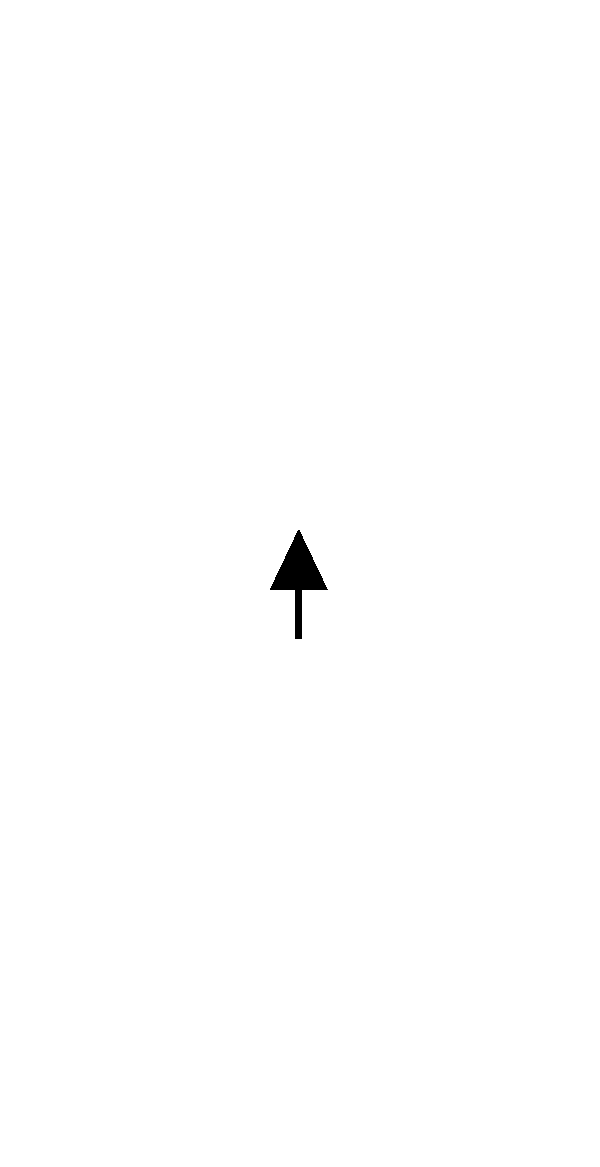
\includegraphics[width=0.2cm]{gfx/arrow.pdf}), with median VI of $4.25$ and $SD=0.07$.}
\label{fig:cremiBboxplot}
\end{figure}

\subsection{CREMI C}

The results of split error correction using focused proofreading and guided proofreading on the CREMI C subvolume are shown in Figure~\ref{fig:cremiCtrails} and~\ref{fig:cremiCboxplot}.

\paragraph{Selection oracle.} With focused proofreading, the initial median VI of 1.75 ($SD=0.086$) is reduced to 1.45 ($SD=0.056$) with 670 accepted corrections out of 2694. Guided proofreading is able to reduce the VI to 1.47 ($SD=0.06$). Here, the oracle accepted 1531 out of 4332 corrections. 

\paragraph{Automatic selection with threshold.} Focused proofreading results in a VI of 4.81 ($SD=0.03$). Guided proofreading with $p_t=0.95$ reduces median VI to 1.57 ($SD=0.081$).

\begin{figure}[t]
\centering
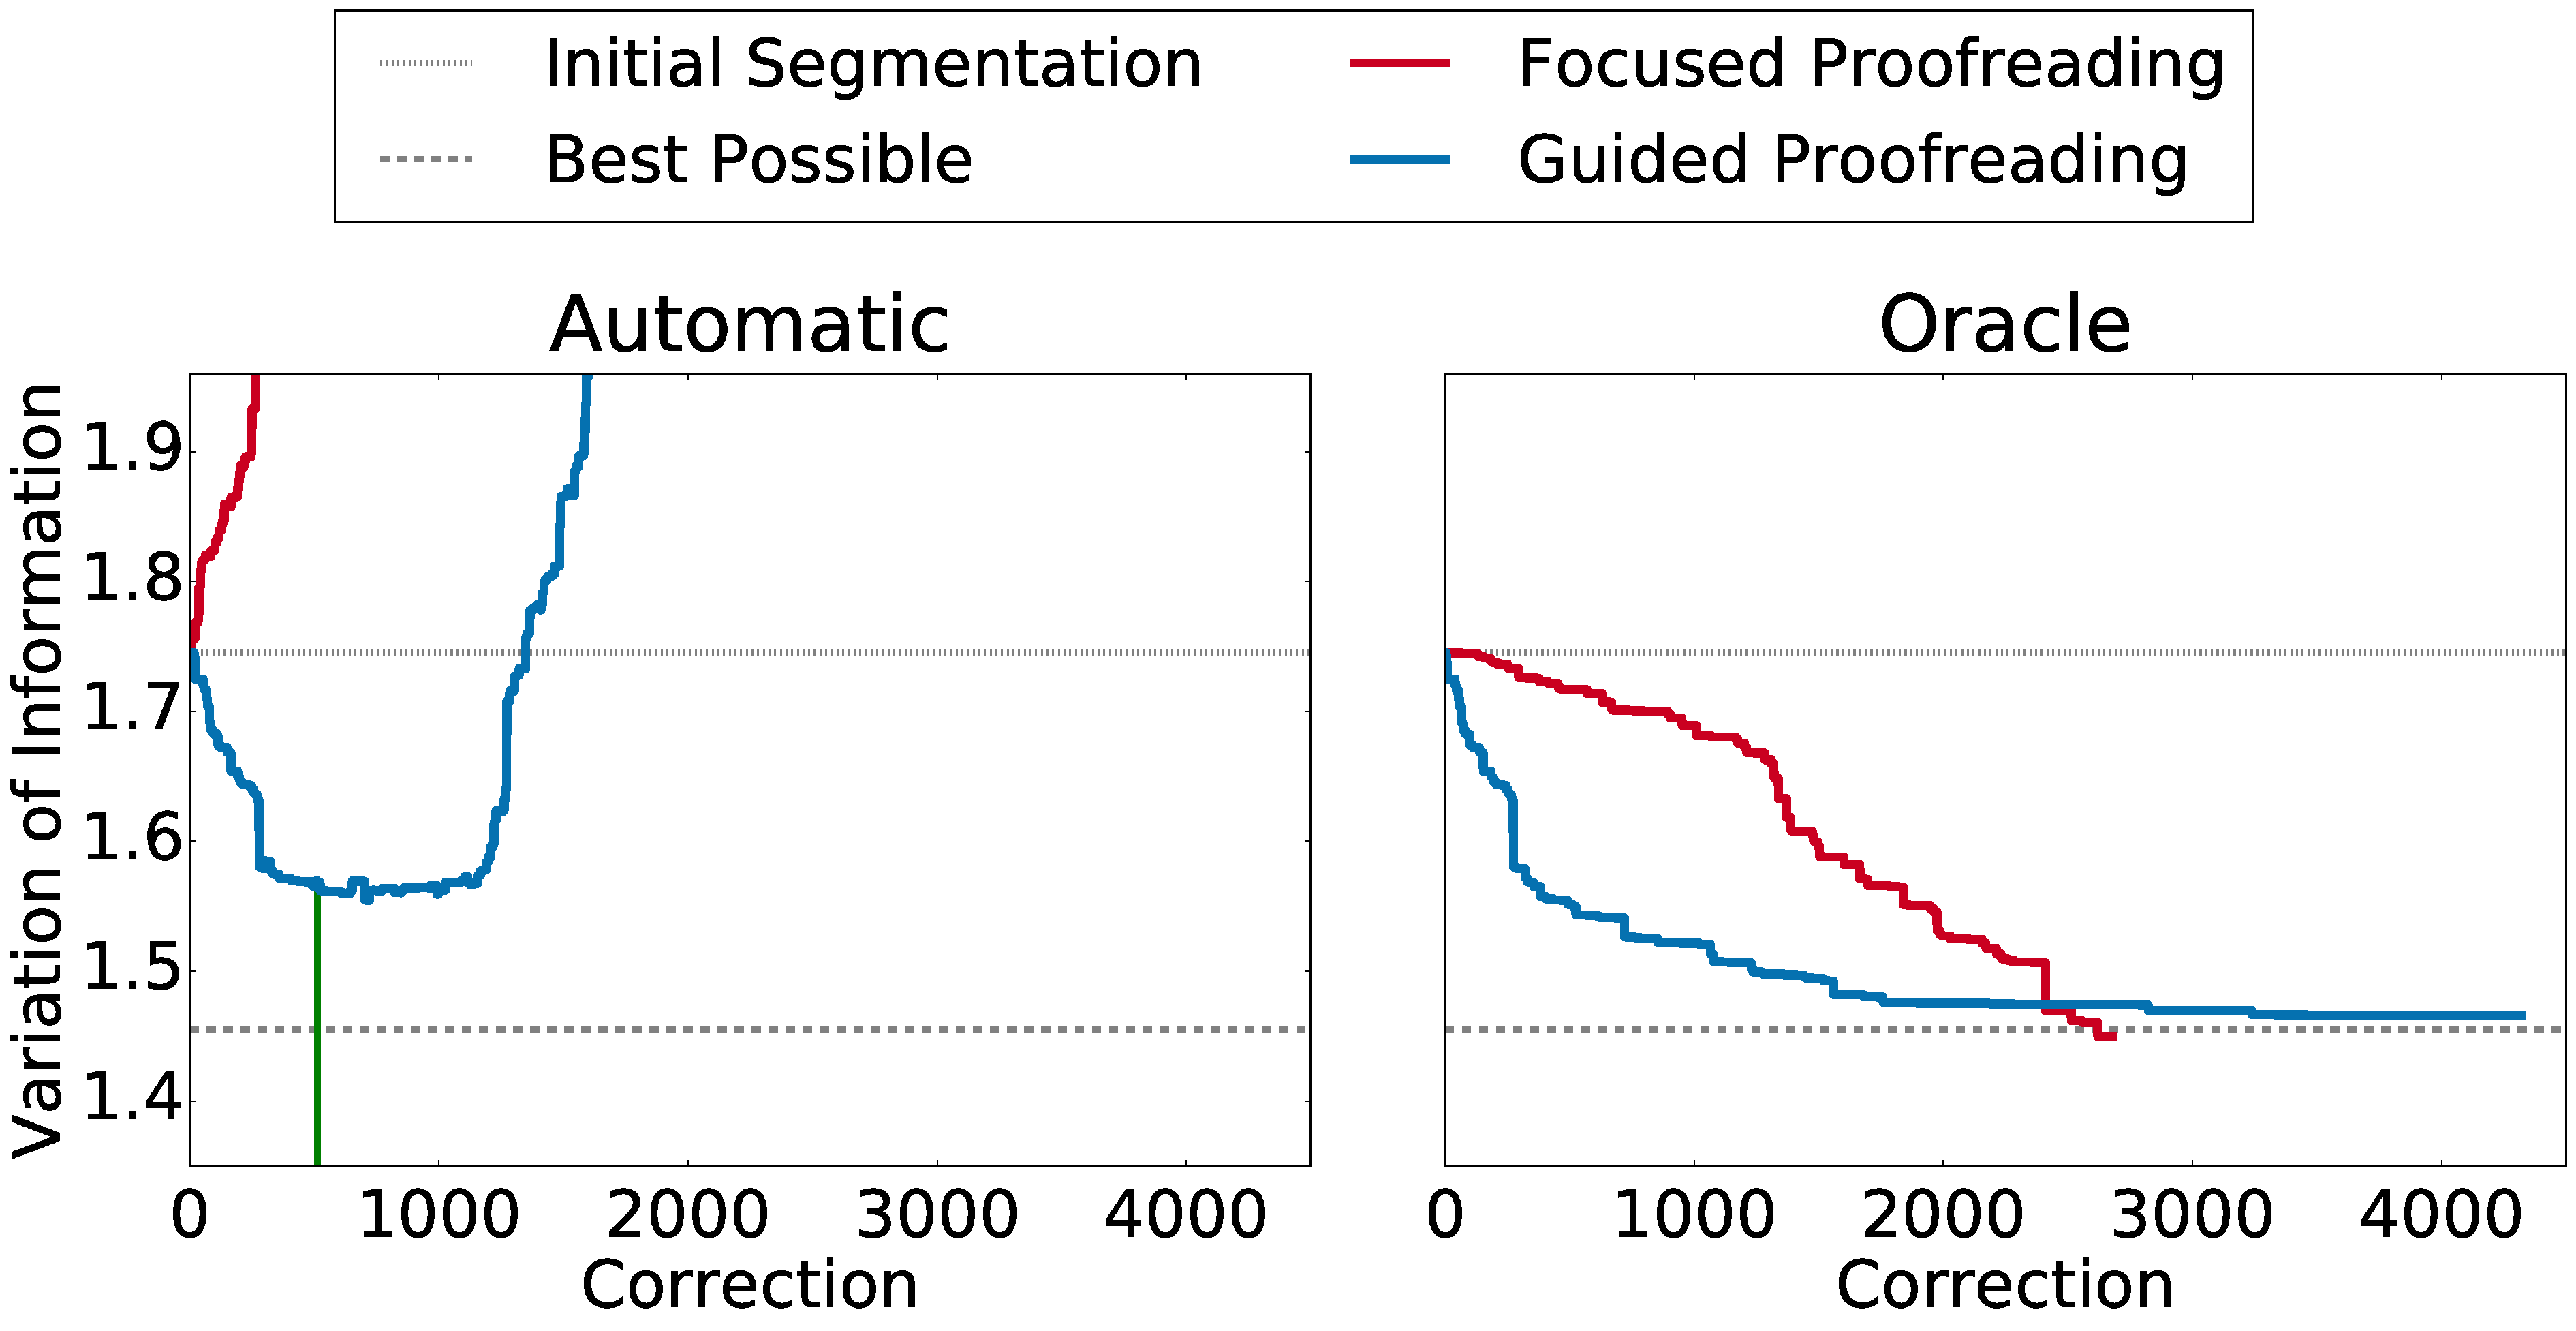
\includegraphics[width=\linewidth]{gfx/cremiC_trails.pdf}
\caption{Performance comparison of Plaza's focused proofreading and our guided proofreading on the CREMI C dataset. Lower VI scores are better. Guided proofreading corrects the initial segmentation faster with less corrections than focused proofreading. The green line shows the automatic threshold $p_t=0.95$.}
\label{fig:cremiCtrails}
\end{figure}

\begin{figure}[t]
\centering
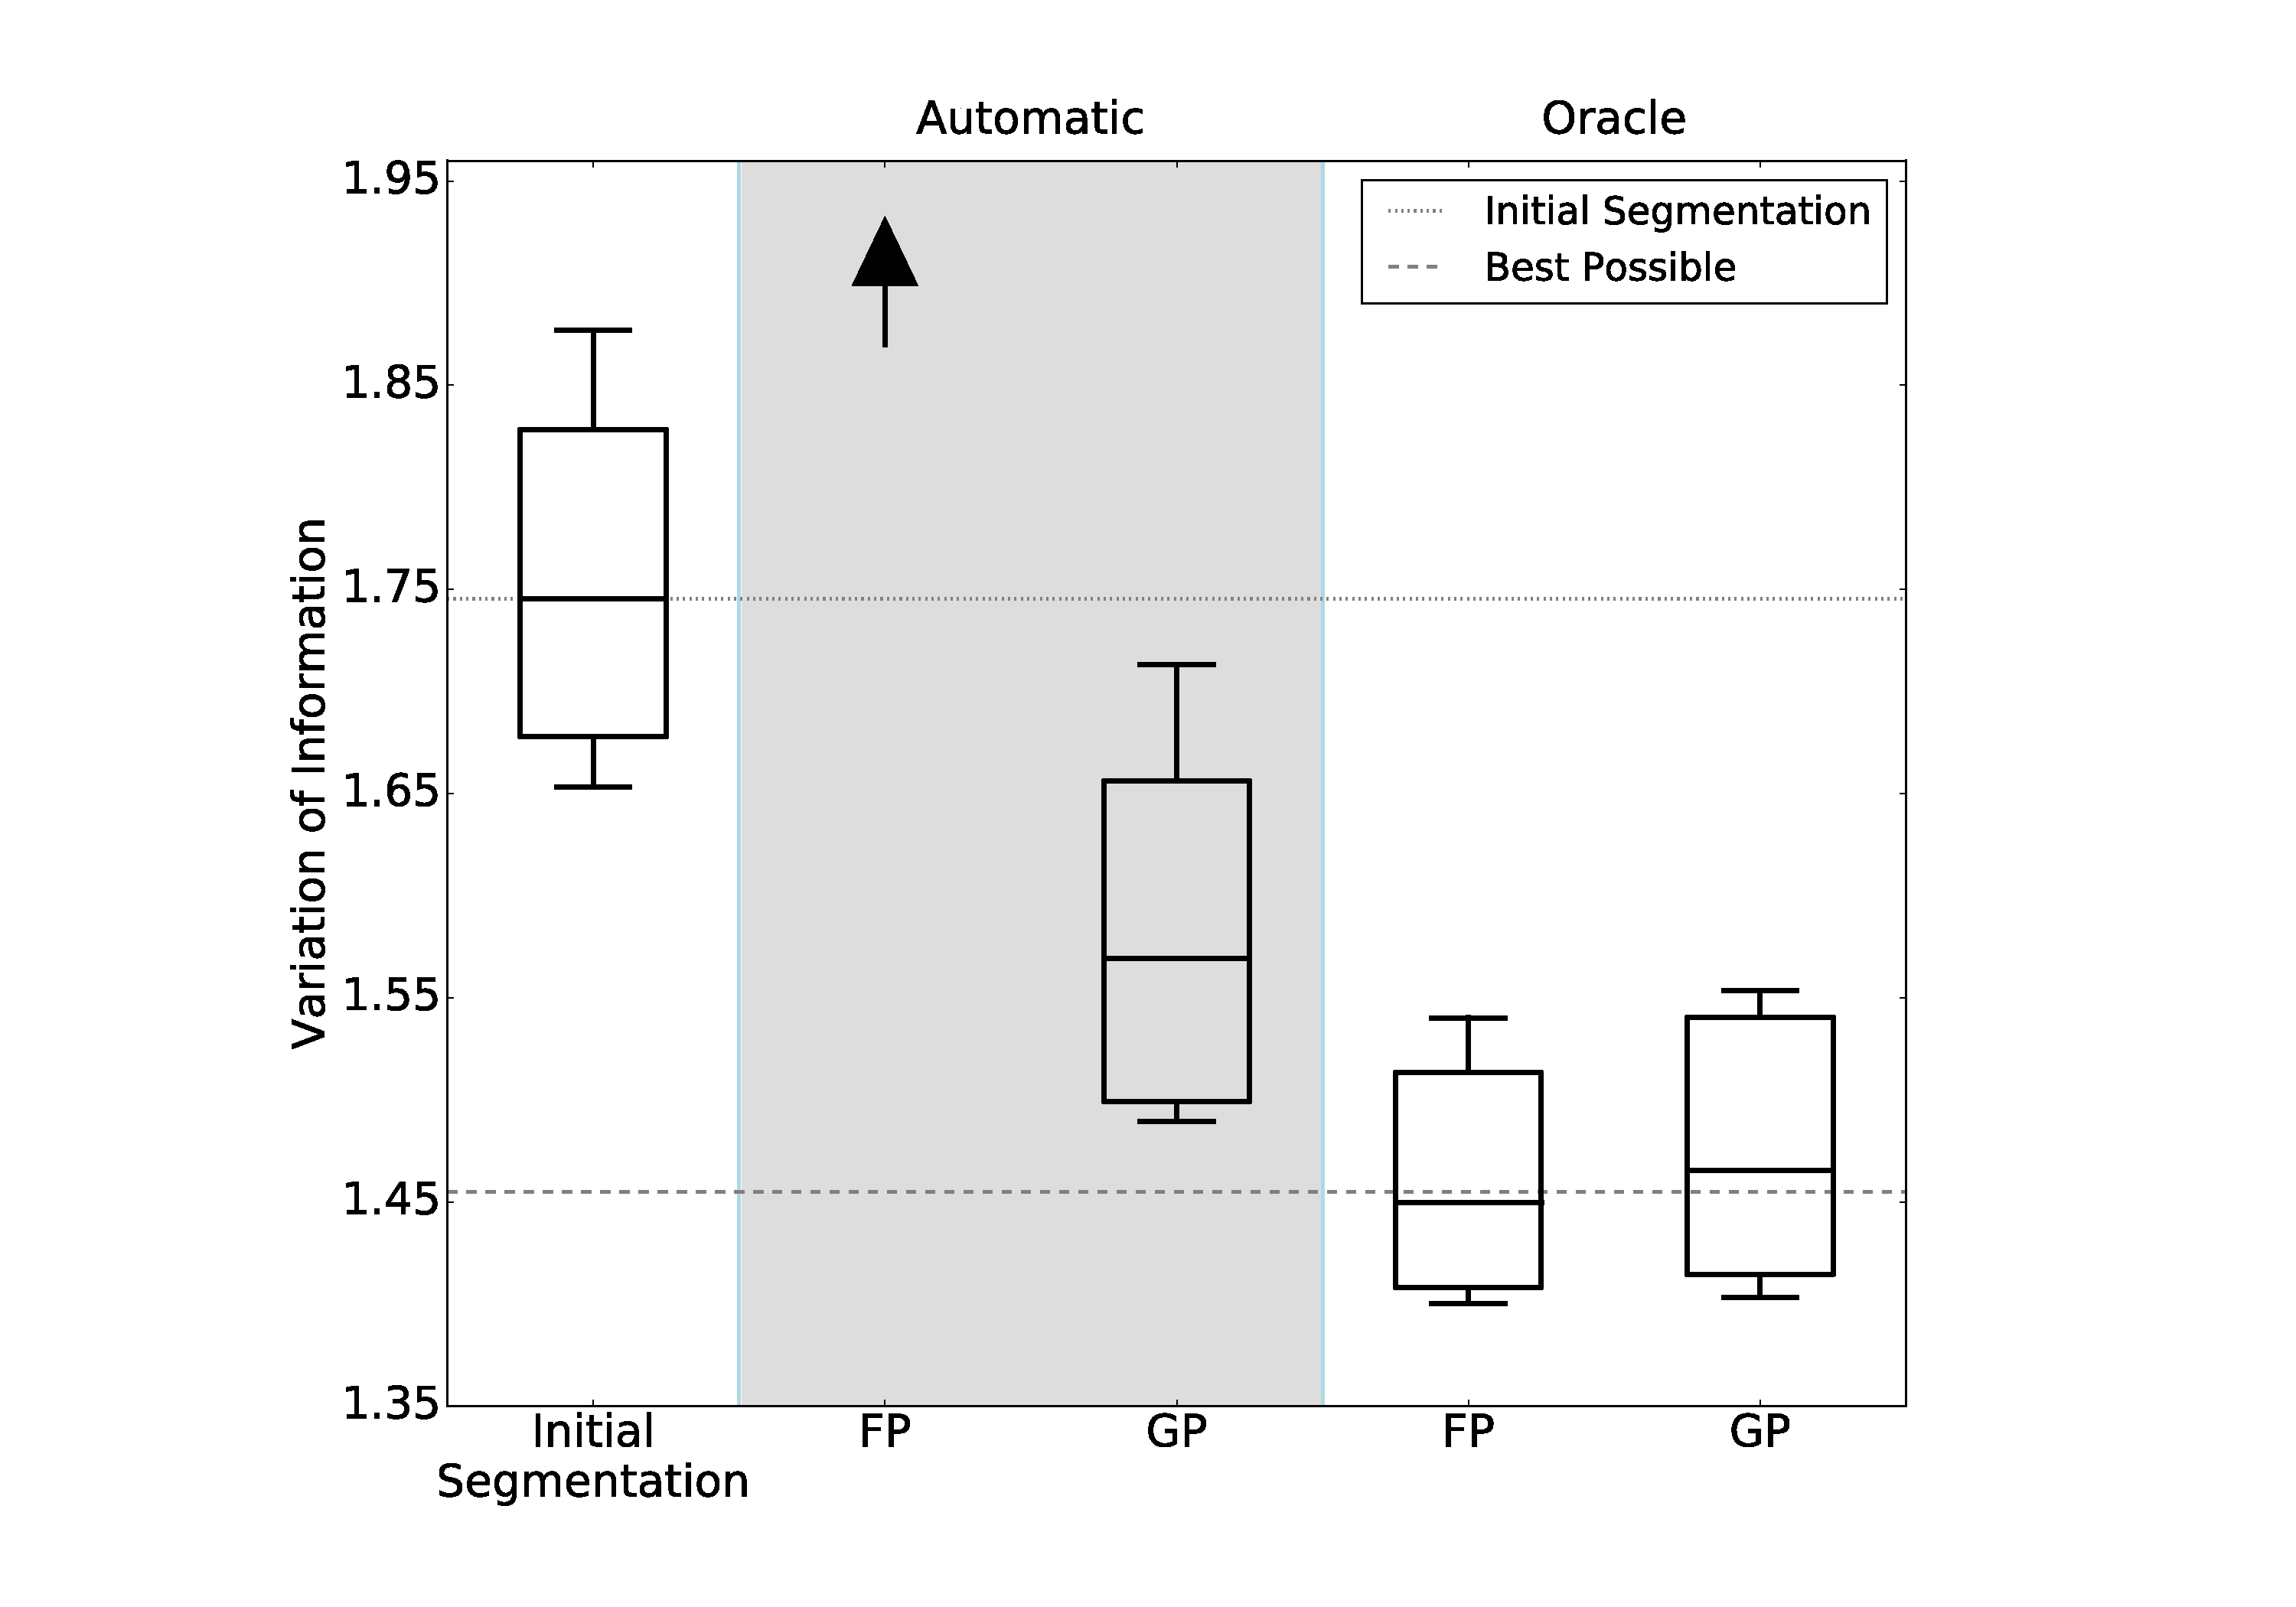
\includegraphics[width=\linewidth]{gfx/cremiCboxplot.pdf}
\caption{VI distributions of guided proofreading (GP) and focused proofreading (FP) output across the CREMI C subvolume, with different error correction approaches. The variation resulting from performance of FP with automatic selection is $3\times$ higher than GP (\protect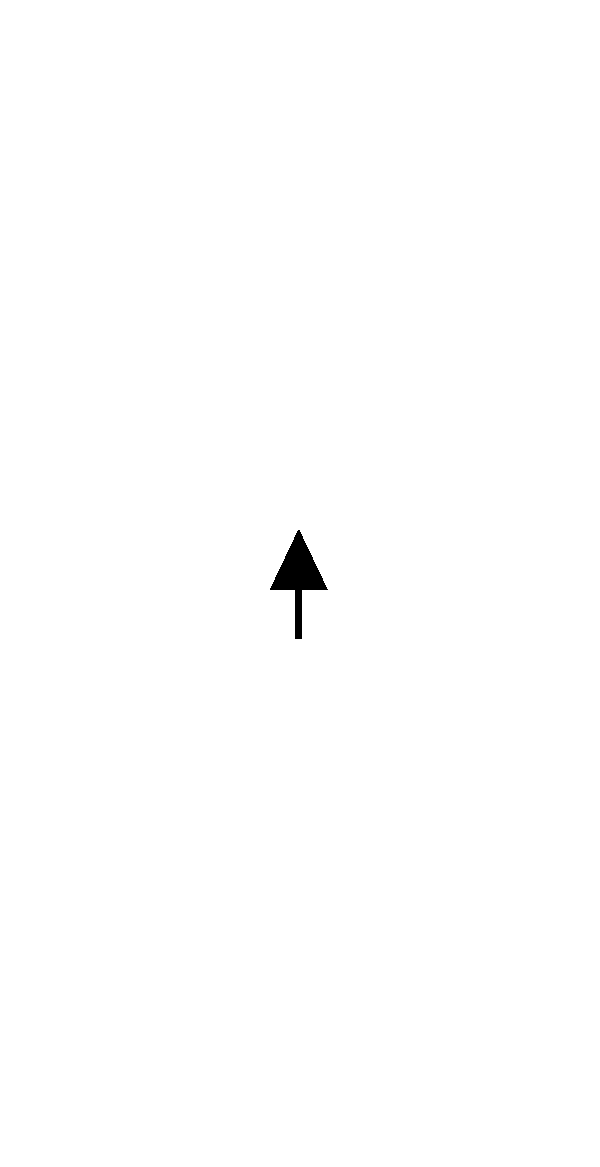
\includegraphics[width=0.2cm]{gfx/arrow.pdf}), with median VI of $4.81$ and $SD=0.08$.}
\label{fig:cremiCboxplot}
\end{figure}